\documentclass[a4paper,twocolumn]{article}

\usepackage{times}
\usepackage[utf8]{inputenc}
\usepackage[portuguese, english]{babel}
\usepackage[a4paper,margin=2cm,columnsep=1cm]{geometry}
\usepackage{authblk}
\usepackage{titlesec}
\usepackage[pdftex]{graphicx}
\usepackage{mathtools}


\begin{document}

\graphicspath{{images/}}
\renewcommand{\abstractname}{\normalsize\bfseries\filcenter ABSTRACT}
\titleformat*{\section}{\normalsize\bfseries\filcenter}
\titleformat*{\subsection}{\small\bfseries\filcenter}
\renewcommand{\refname}{\normalsize\bfseries\filcenter REFERÊNCIAS}
\renewcommand{\figurename}{\small Figura}
\newcommand{\figureref}[1]{\textit{Figura \ref{fig:#1}}}
\newcommand{\equationref}[1]{\textit{Equação \ref{eq:#1}}}
\newcommand{\bigsum}{\displaystyle\sum}

\title{\textbf{Modulações Digitais BPSK e QPSK}}
\author{\textit{Eduardo M. B. de A. Tenório\textsuperscript{1}, Diogo B. da Silva\textsuperscript{2}, Gilberto P. de F. Sobrinho\textsuperscript{2}, Rodrigo J. C. Q. Peixe\textsuperscript{3} e Daniel C. Cunha\textsuperscript{1}}}
\affil{Centro de Informática, Universidade Federal de Pernambuco\\
Recife, PE, Brasil -- www.cin.ufpe.br\\
\small\textsuperscript{1}\texttt{\{embat,dcunha\}@cin.ufpe.br}\\
\small\textsuperscript{2}\texttt{\{diogo.bs1,gibapfarias\}@hotmail.com}\\
\small\textsuperscript{3}\texttt{rodrigo.peixe@gmail.com}}
\date{Agosto, 2014}

\maketitle


\begin{abstract}
\begin{itshape}
Este documento é uma descrição dos resultado obtidos na implementação do projeto básico \#2 da disciplina Princípios de Comunicação, ministrada pelo professor Daniel Cunha. Inicialmente é falado brevemente sobre modulação digital. Em seguida são descritas maneiras de modificar o sinal transmitido e logo mais são detalhadas as modulações utilizadas. Por fim são mostradas alguns gráfico da taxa de erro de bit pela relação sinal-ruído, comprovando o que foi explicado previamente.\\

\noindent\textbf{palavras-chave}: modulação digital, bpsk, qpsk, AWGN, Rayleigh
\end{itshape}
\end{abstract}


\section{INTRODUÇÃO}

Este projeto teve como objetivo a implementação de uma simulação computacional de sistemas de comunicação digitais, utilizando as modulações Phase-Shift Keying (PSK) e Quadrature Amplitude Modulation (QAM). A forma de avaliar o desempenho de cada tipo de modulação foi através da taxa de erro de bit versus a relação sinal-ruído. Foi efetuada uma comparação dos desempenhos da curva analítica e da curva simulada, utilizando um canal com Ruído Aditivo Gaussiano Branco (AWGN) e Desvanecimento Rayleigh.

As modulações especificadas foram a BPSK (2-PSK) e QPSK (4-PSK), subtipos da modulação PSK, e 16-QAM e 64-QAM, subtipos da modulação QAM. O empreendimento obteve sucesso parcial, com a implementação da simulação para as modulações do tipo $M$-PSK, a adição do AWGN e o Desvanecimento Rayleigh.

O restante do documento está organizado da seguinte forma: na seção 2 há um descrição sucinta do AWGN. O Desvanecimento Rayleigh é descrito na seção 3. A seção 4 fala sobre a modulação PSK, detalhando a BPSK e a QPSK. Na seção 5 é descrita a simulação. A seção 6 apresenta a conclusão do trabalho e, por fim, as referências.

Todo o código utilizado para este trabalho, bem como imagens e demais documentos (este incluso) encontram-se num repositório no Github, disponível através da url \textit{https://github.com/embatbr/psk-qam}. A linguagem utilizada foi Python, versão 3.4.


\section{ADDITIVE WHITE GAUSSIAN NOISE}

Ruído é um sinal de natureza aleatória que interfere no sinal transmitido, algumas vezes ocasionando uma diferença na detecção da mensagem (no caso de uma mensagem binária, por exemplo, alguns bits podem ser trocados durante a transmissão), o que é considerado um erro. Uma forma de saber o quão resistente a ruídos é um sinal é a relação sinal-ruído (SNR, de \textit{signal-to-noise ratio}), que nada mais é que uma razão entre a potência do sinal enviado e a potência do ruído.

O AWGN é um ruído aditivo (ou seja, seu valor é adicionado ao valor do sinal), branco (todas as faixas de frequência possuem a mesma potência) e cuja amplitude segue uma distribuição gaussiana (distribuição normal). O termo ``ruído branco" é derivado do conceito de luz branca, que existe em todo o espectro de frequência. O ruído é dado pela equação

\begin{equation}
    \label{eq:awgn}
    n(x) = \frac{1}{\sigma \sqrt{2\pi}} e^{- \frac{(x - \mu)^2}{2\sigma^2}}
\end{equation}

\noindent com $\mu = 0$ e $\sigma^2 = \frac{N_0}{2}$. O sinal recebido é dado por $y(t) = s(t) + n(t)$, onde $s(t)$ é o sinal transmitido e $n(t)$ é o ruído.

A probabilidade de erro de bit, $P_b$ de um sinal em um canal com AWGN é dada pela equação abaixo. Para cada valor de SNR, o valor correspondente do Bit Error Rate (BER) é o $P_b$.

\begin{equation}
    \label{eq:bit_error_prob}
    P_b = \frac{1}{2}erfc(\sqrt{\frac{E_b}{N_0}})
\end{equation}


\section{DESVANECIMENTO RAYLEIGH}

Modelo estocástico de propagação no ambiente de um sinal de rádio, que ocorre quando não há ``visão" direta entre a fonte e o receptor. Como a propagação é indireta, o sinal apresenta um decaimento (desvanecimento) devido à reflexão, que varia aleatoriamente, de acordo com a distribuição Rayleigh, descrita pela equação

\begin{equation}
    \label{eq:rayleigh_dist}
    p(h) = \frac{h}{\sigma^2}e^\frac{-h^2}{2\sigma^2}
\end{equation}

A probabilidade de erro de bit num canal com AWGN e Desvanecimento Rayleigh é dada pela equação a seguir, derivada da \equationref{bit_error_prob}.

\begin{equation}
    \label{eq:rayleigh_bit_error_prob}
    P_b = \frac{1}{2}(1 - \sqrt{\frac{\frac{E_b}{N_0}}{\frac{E_b}{N_0} + 1}})
\end{equation}


\section{MODULAÇÃO PSK}

Phase-shift keying (ou \textit{chaveamento por descolamento de fase}) é um esquema de modulação digital que atua alterando a fase da onda portadora (vide figura abaixo).

\begin{figure}[h]
    \label{fig:psk_mod}
    \centering
    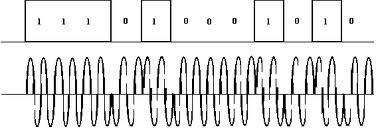
\includegraphics[scale=0.55]{psk-mod}
    \caption{\textit{Modulação PSK. Veja como a fase da portadora muda ao trocar o bit.}}
\end{figure}

Comumente é chamado de modulação $M$-PSK, onde $M$ indica o número de símbolos (2, 4, 8\dots). As duas modulações estudadas para este projeto foram a binary phase-shift keying (BPSK) e a quadrature phase-shift keying (QPSK), ambas descritas nas subseções a seguir.

\subsection{BPSK}

A BPSK ou 2-PSK é um tipo de PSK no qual cada símbolo é representado por apenas um bit. Dado $k = \sqrt{M}$ o número de bits por símbolo, para o BPSK, $k = 1$. Sua equação no domínio do tempo é

\begin{equation}
    \label{eq:bpsk_time}
    s_n(t) = \sqrt{\frac{2E_b}{T_b}}cos(2\pi f_c t + \pi(1 - n)), n = 0, 1.
\end{equation}

\noindent e seus (dois) possíveis em forma vetorial (apenas no eixo real) são mostrados na figura a seguir

\begin{figure}[h]
    \label{fig:bpsk_vector}
    \centering
    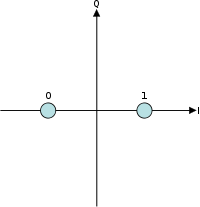
\includegraphics[scale=0.55]{bpsk-vector}
    \caption{\textit{Possíveis valores do sinal BPSK.}}
\end{figure}

\subsection{QPSK}

Similarmente ao BPSK, o QPSK é uma modulação PSK, mas com quatro possíveis valores (e dois bits por símbolo). Sua representação vetorial é mostrada na figura a seguir

\begin{figure}[h]
    \label{fig:qpsk_vector}
    \centering
    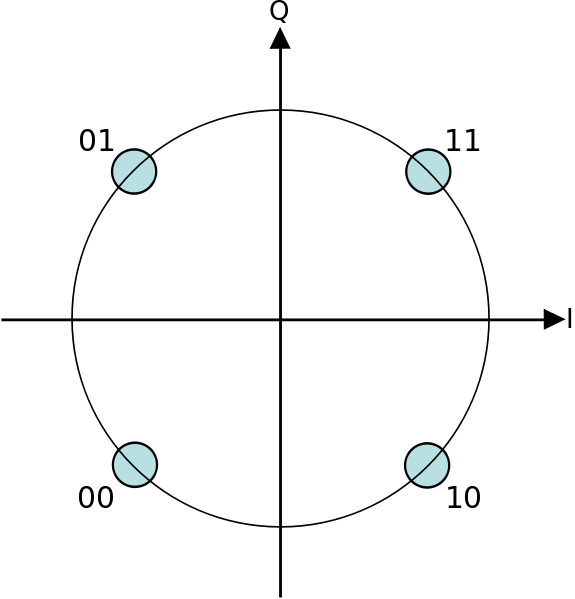
\includegraphics[scale=0.20]{qpsk-vector}
    \caption{\textit{Possíveis valores do sinal QPSK.}}
\end{figure}

\noindent e sua equação no domínio do tempo é

\begin{equation}
    \label{eq:qpsk_time}
    s_n(t) = \sqrt{\frac{2E_b}{T_b}}cos(2\pi f_c t + \frac{\pi}{4}(2n - 1)), n = 1, 2, 3, 4.
\end{equation}


\section{SIMULAÇÃO}

A simulação foi efetuada gerando aleatoriamente uma string de bits com comprimento $l$, onde $l$ é uma ordem de grandeza maior que o denominador do $P_b$ correspondente da curva analítica calculada para um determinado valor SNR. Por exemplo, se $P_b$ for da ordem de $10^{-3}$, então a string de bits possui comprimento $10^4$.

Para cada modulação (BPSK e QPSK) foram calculados 11 gráficos. O primeiro mostra a curva analítica do erro esperado em vermelho e a curva do BER simulado em azul. Os gráficos seguintes foram calculados com várias escalas de Desvanecimento Rayleigh (de 0.1 a 1 e incremento de 0.1). Percebe-se que com o aumento da escala, o desvanecimento diminui e a curva simulada aproxima-se da analítica. O sinal recebido é dado pela equação

\begin{equation}
    \label{eq:signal_rayleigh}
    r = \frac{hs + n}{h}
\end{equation}

\noindent onde $h$ representa o Desvanecimento Rayleigh. Ao final do documento são mostradas alguns gráficos gerados execução do programa desenvolvido.


\section{CONCLUSÃO}

Este trabalho permitiu conhecer de maneira mais detalhada como funcionam as modulações digitais, principalmente a PSK. O que foi aprendido teve reflexo no exame da disciplina, levando os integrantes do grupo a apresentarem um bom desempenho devido ao tempo dedicado à implementação do código. Pode-se dizer que os integrantes apenas aprenderam o conteúdo devido a este projeto.

Também foi produtivo engajar-se numa atividade de simulação de sinais reais, além de ter sido necessário aprender a utilizar ferramentas até então desconhecidas.

Infelizmente não foi possível completar o escopo, tanto pelas dificuldades inerentes ao projeto (complexidade do assunto, tempo compartilhado com outras disciplinas), quanto pela diminuição da equipe efetiva.


\begin{thebibliography}{9}
    \bibitem{sklar_book}
        B. Sklar,
        ``Fading Channels,"
        in \textit{Digital Communications: Fundamentals and Applications,}
        2nd ed.
        Tarzana, California: University of California, Los Angeles,
        2001, ch. 15, pp. 944-1011.

    \bibitem{comm_theory}
        http://wiki.scipy.org/Cookbook/CommTheory

    \bibitem{dsplog_1}
        http://www.dsplog.com/2007/08/05/bit-error-probability-for-bpsk-modulation/

    \bibitem{dsplog_2}
        http://www.dsplog.com/2008/08/10/ber-bpsk-rayleigh-channel/
\end{thebibliography}


\begin{figure}[h]
    \label{fig:2-psk_awgn}
    \centering
    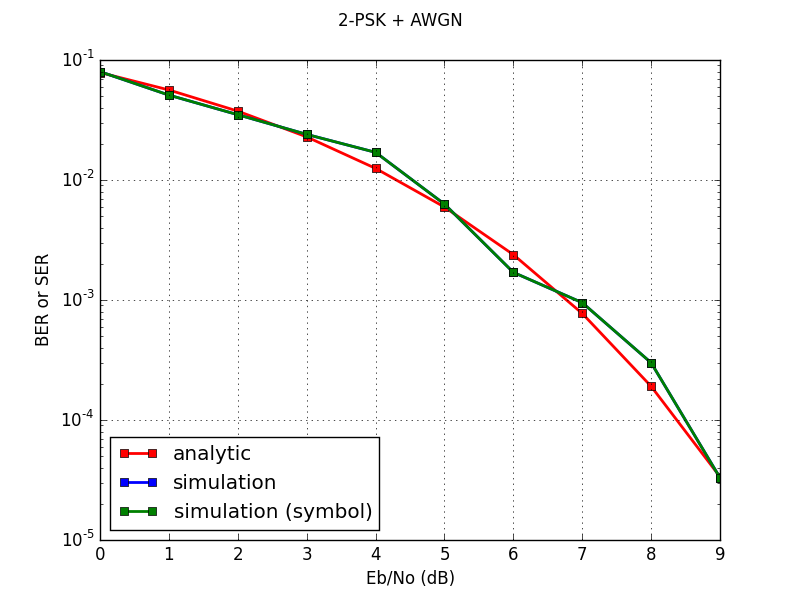
\includegraphics[scale=0.40]{2-psk_awgn}
    \caption{\textit{Curvas analítica e simulada para $P_b$ versus SNR com AWGN. Note que a curva de erro de bit e a curva de erro de símbolo são a mesma ($k = 1$).}}
\end{figure}

\begin{figure}[h]
    \label{fig:2-psk_awgn_10_rayleigh}
    \centering
    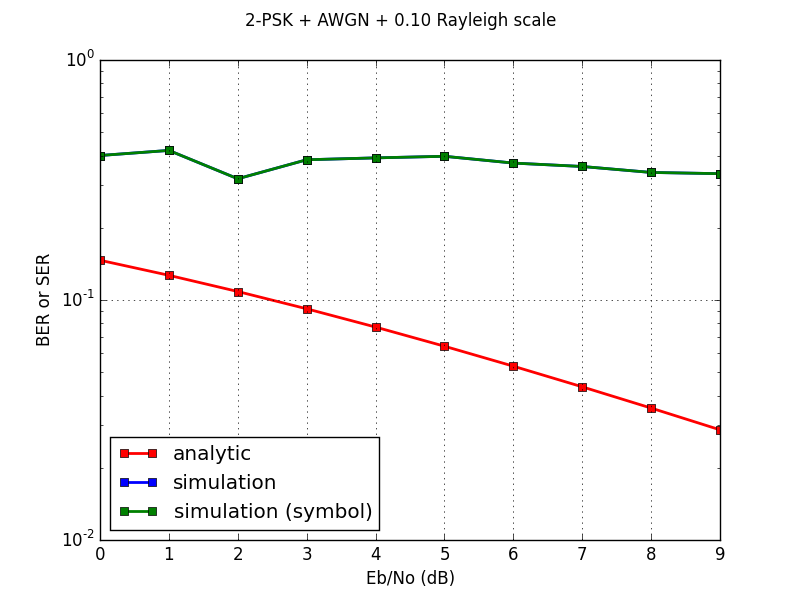
\includegraphics[scale=0.40]{2-psk_awgn_10_rayleigh}
    \caption{\textit{Curvas analítica e simulada para $P_b$ versus SNR com AWGN e Desvanecimento Rayleigh com escala 0.1.}}
\end{figure}

\begin{figure}[h]
    \label{fig:2-psk_awgn_100_rayleigh}
    \centering
    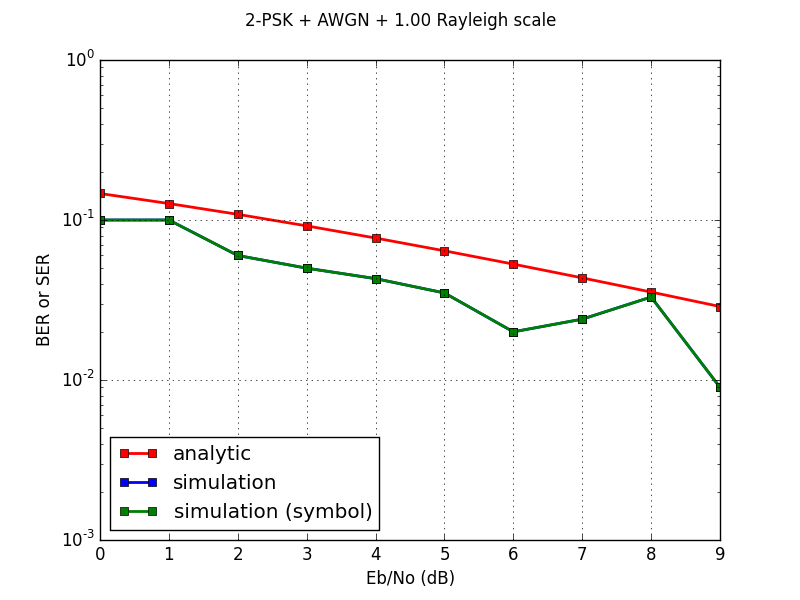
\includegraphics[scale=0.40]{2-psk_awgn_100_rayleigh}
    \caption{\textit{Curvas analítica e simulada para $P_b$ versus SNR com AWGN e Desvanecimento Rayleigh com escala 1.}}
\end{figure}

\begin{figure}[h]
    \label{fig:4-psk_awgn}
    \centering
    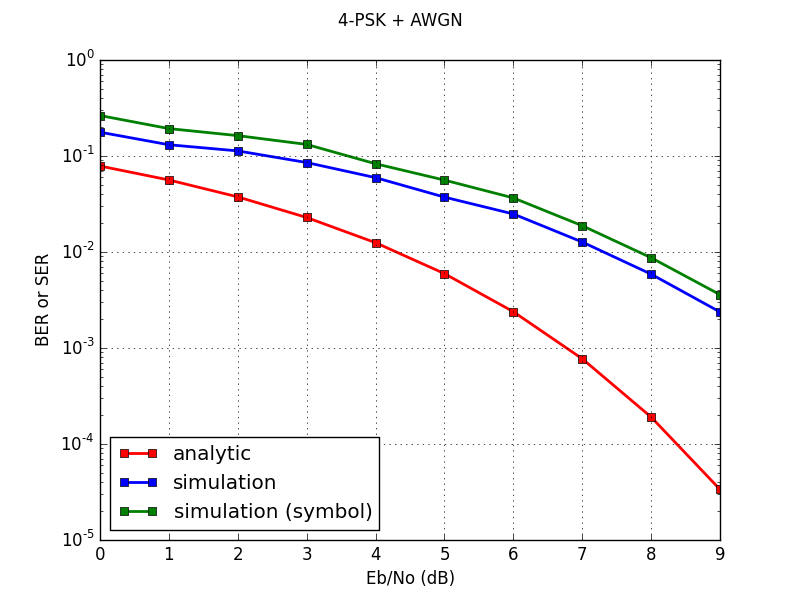
\includegraphics[scale=0.40]{4-psk_awgn}
    \caption{\textit{Curvas analítica e simulada para $P_b$ versus SNR com AWGN.}}
\end{figure}

\begin{figure}[h]
    \label{fig:4-psk_awgn_10_rayleigh}
    \centering
    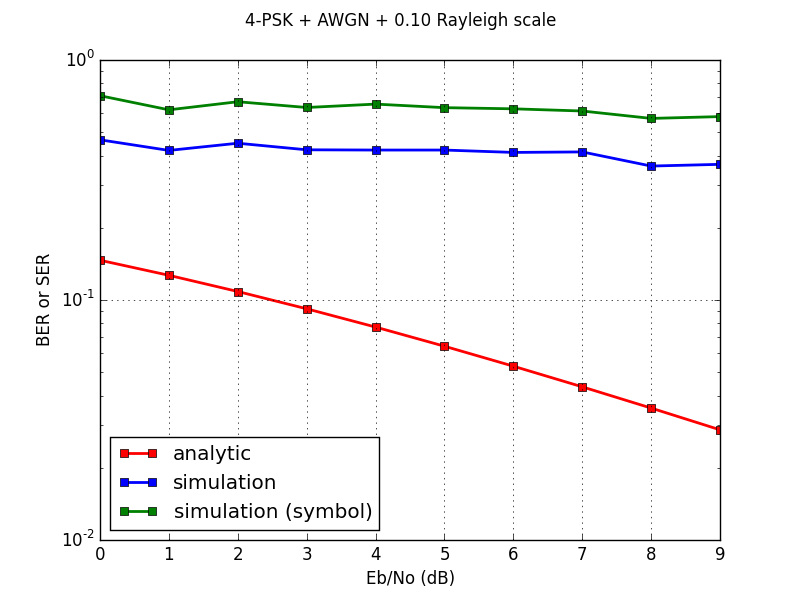
\includegraphics[scale=0.40]{4-psk_awgn_10_rayleigh}
    \caption{\textit{Curvas analítica e simulada para $P_b$ versus SNR com AWGN e Desvanecimento Rayleigh com escala 0.1.}}
\end{figure}

\begin{figure}[h]
    \label{fig:4-psk_awgn_100_rayleigh}
    \centering
    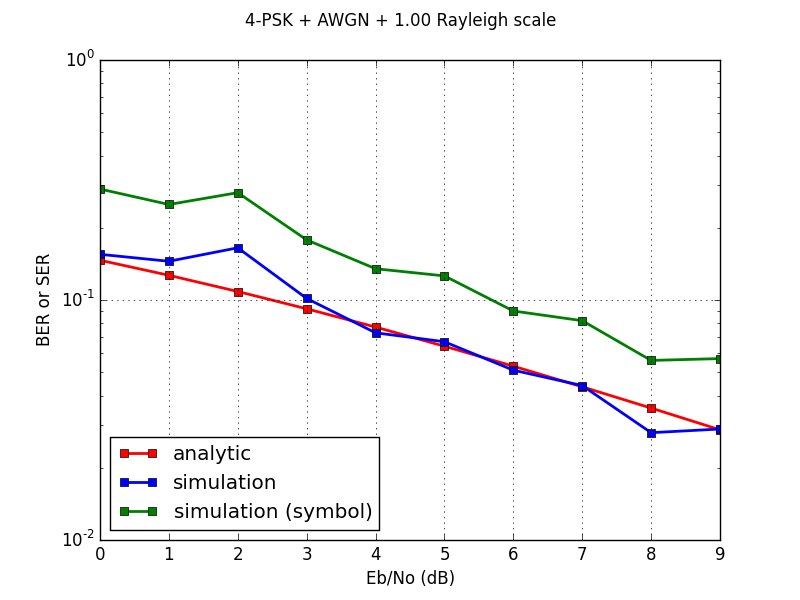
\includegraphics[scale=0.40]{4-psk_awgn_100_rayleigh}
    \caption{\textit{Curvas analítica e simulada para $P_b$ versus SNR com AWGN e Desvanecimento Rayleigh com escala 1.}}
\end{figure}

\end{document}